\chapter{Gene Cloning}

\section{Genetic Engineering Applications}
\bd{Plants}\\[.1in]
A wide variety of different alterations has been made plants affecting not just their yields but also multiple resistances.\\[.2in]
\bd{Pharmaceutical industry}\\[.1in]
Product like recombinant insulin or variants, recombinant GCSF\footnote{prevents infections during cancer
chemotherapy}, humanising therapeutic antibodies are developed.\\[.2in]
\bd{Research}
\begin{enumerate}[noitemsep]
    \item \udl{molecular biology} enzyme production, time/location functional studies
    \item developmental biology: GFP (and related) fusion proteins
    \item gene knock-out/in libraries
\end{enumerate}

\section{Cloning Vectors for use in E. coli}
Derived from plasmids\footnote{a genetic structure in a cell that can replicate independently of the chromosomes} and bacteriophage\footnote{phage for short: a virus which parasitizes a bacterium by infecting it and reproducing inside it.}. Important parts includes:
\begin{itemize}[noitemsep]
    \item origin of replication
    \item selectable marker
    \item multiple cloning site (MCS)
\end{itemize}

\subsection{Typical workflow for making recombinant DNA}
\begin{figure}[h]
\centering
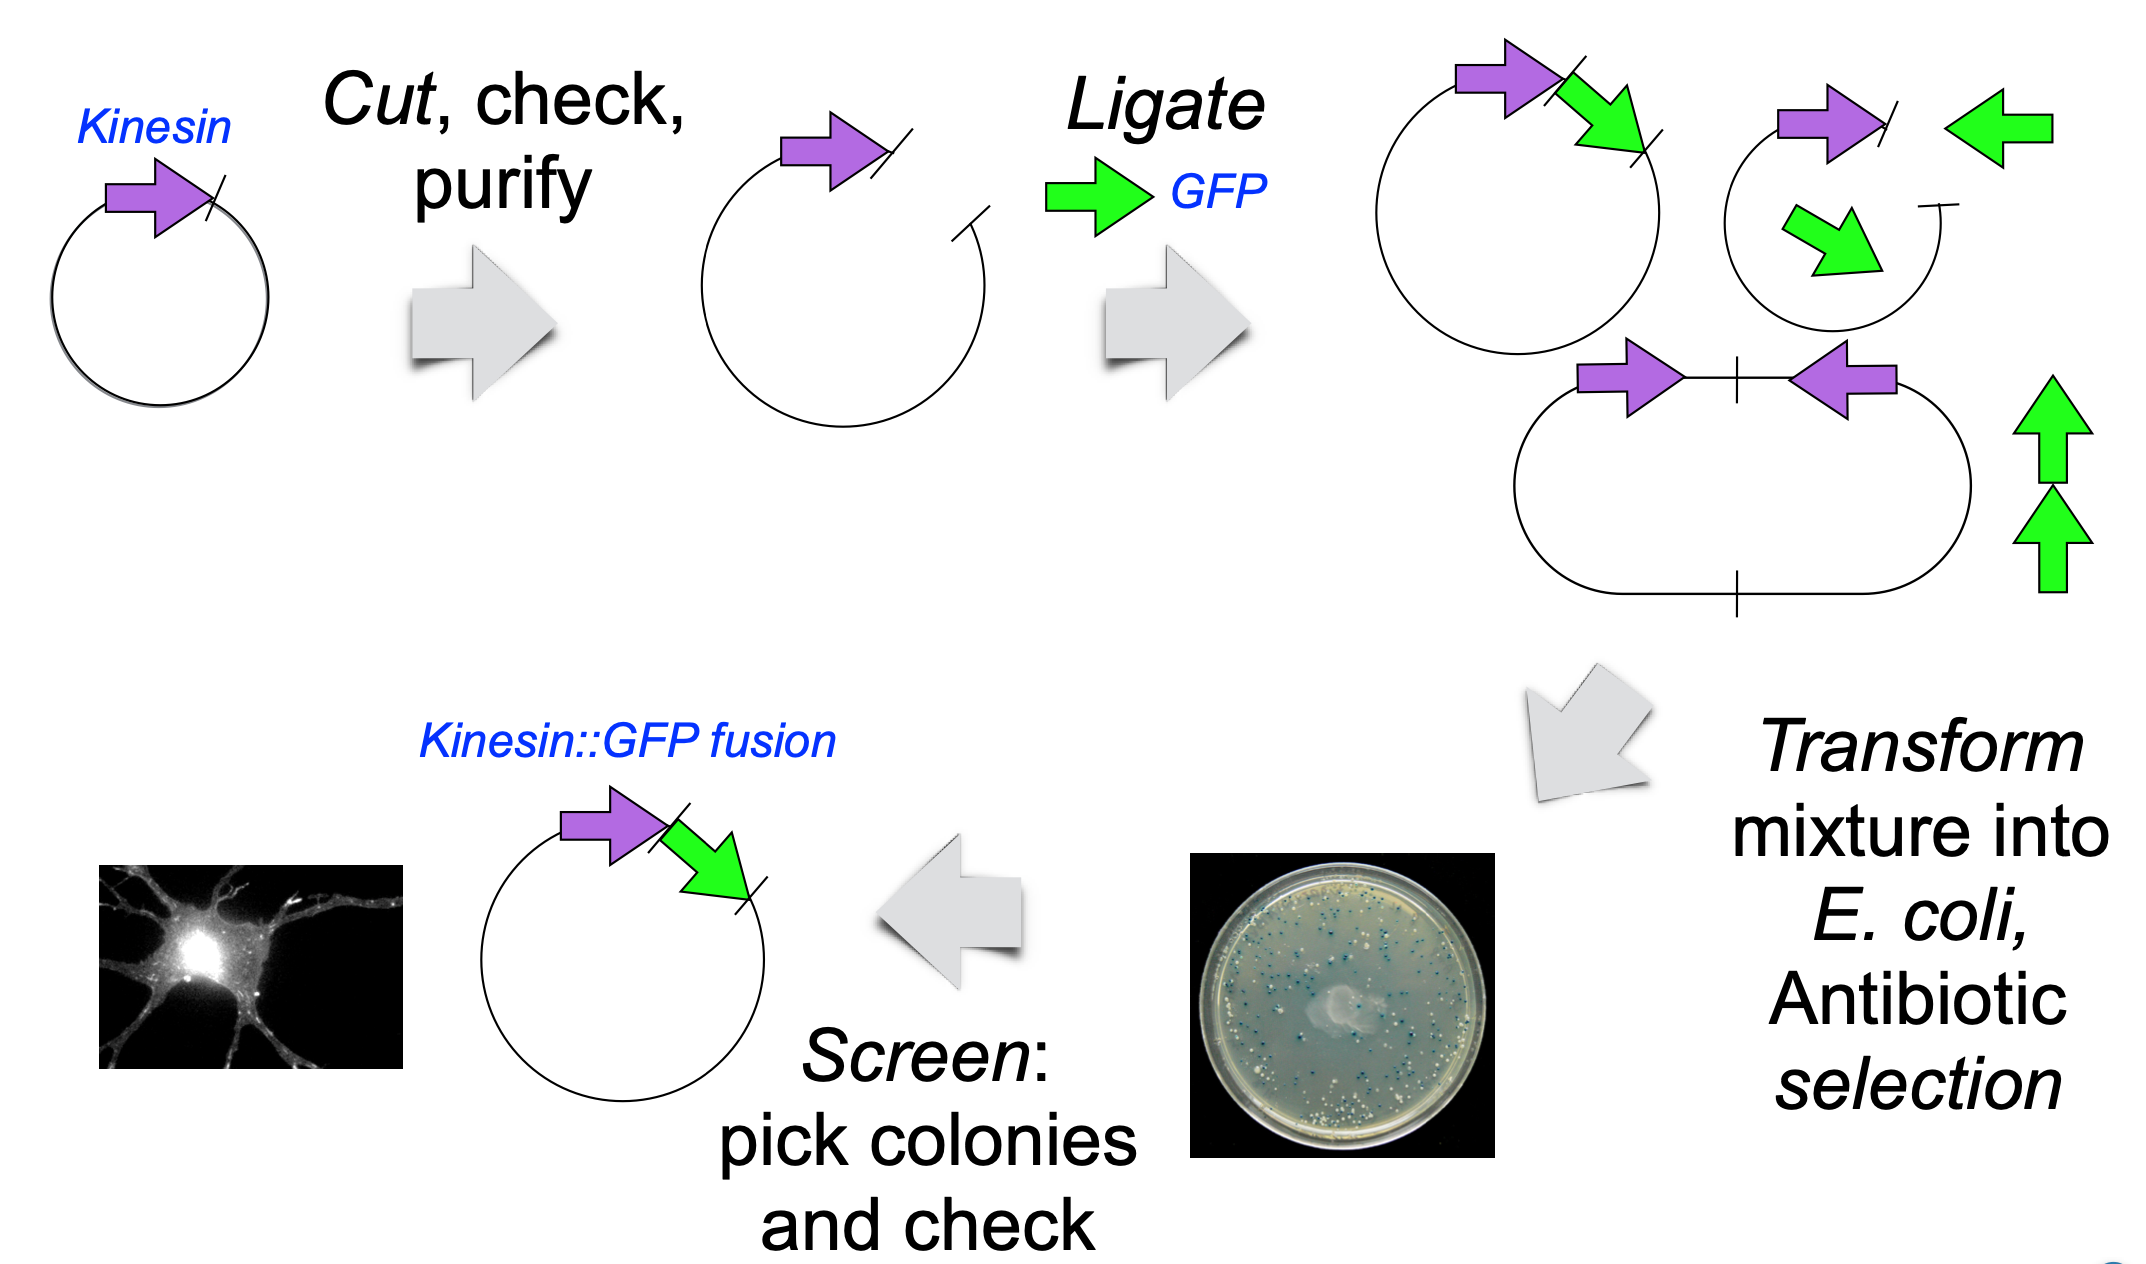
\includegraphics[width=0.8\textwidth]{images/lecture4-1.png}\\[.2in]
\caption{Typical workflow for making recombinant DNA} 
\end{figure}
\subsection{Distinguish between single clones and libraries of clones}
\bd{Make one clone}\\
For example, fusing one gene (GFP) to another (kinesin)\\[.2in]
\bd{Making a library of clones}\\
For example, cloning a set of fragments representing all genes expressed in a tissue.
\subsection{Bacterial plasmids and phage}
Recall prokaryotic horizontal gene transfer via conjugation (moves plasmids) or transduction by phage.
\subsection{Selectable markers}
\begin{itemize}[noitemsep]
    \item Ampicillin: amp\textsuperscript{r}
    \item Kanamycin: kan\textsuperscript{r}
    \item Tetracyclines: tet\textsuperscript{r}
    \item Chloramphenicol: cap\textsuperscript{r}
\end{itemize}
\subsection{Cutting DNA: Restriction enzymes}
\bd{Restriction enzymes cut DNA}
\begin{itemize}
    \item It cuts \udl{specific sequence motif}\footnote{distinctive sequence on a protein or DNA, having a three-dimensional structure that allows binding interactions to occur.}.
    \item the motif is often \udl{palindromic}.
    \item Bacterial defence mechanism: restriction enzymes only cut unmethylated DNA, for example, invading viral DNA.
    \item Chromosomal DNA is protected by a DNA methylase that methylates the motif.
\end{itemize}
\bd{Sticky and Blunt cut}
\begin{enumerate}
    \item \bd{Blunt Cut}: The cuts of the DNA strand are opposite to each other.
    \item \bd{Sticky Overhang}: After cutting and separation, there is a short 4 base extension.
    \begin{enumerate}
        \item Sticky: 5' overhang (extension on 3')
        \item Sticky: 3' overhang (extension on 5')
    \end{enumerate}
\end{enumerate}
\subsection{Pasting DNA: DNA Ligase}
\begin{itemize} 
    \item DNA ligase rejoins cut DNA strands.
    \item Ligase works on \udl{correctly base-paired} sticky ends.
    \item Ligase can also join blunt-ended DNA, but less efficiently.
\end{itemize}
\subsection{Recombinant DNA}
The figure \ref{Fig4-2} illustrates the sequence dependent cleavage and assembly of DNA.
\begin{figure}[h]
\centering
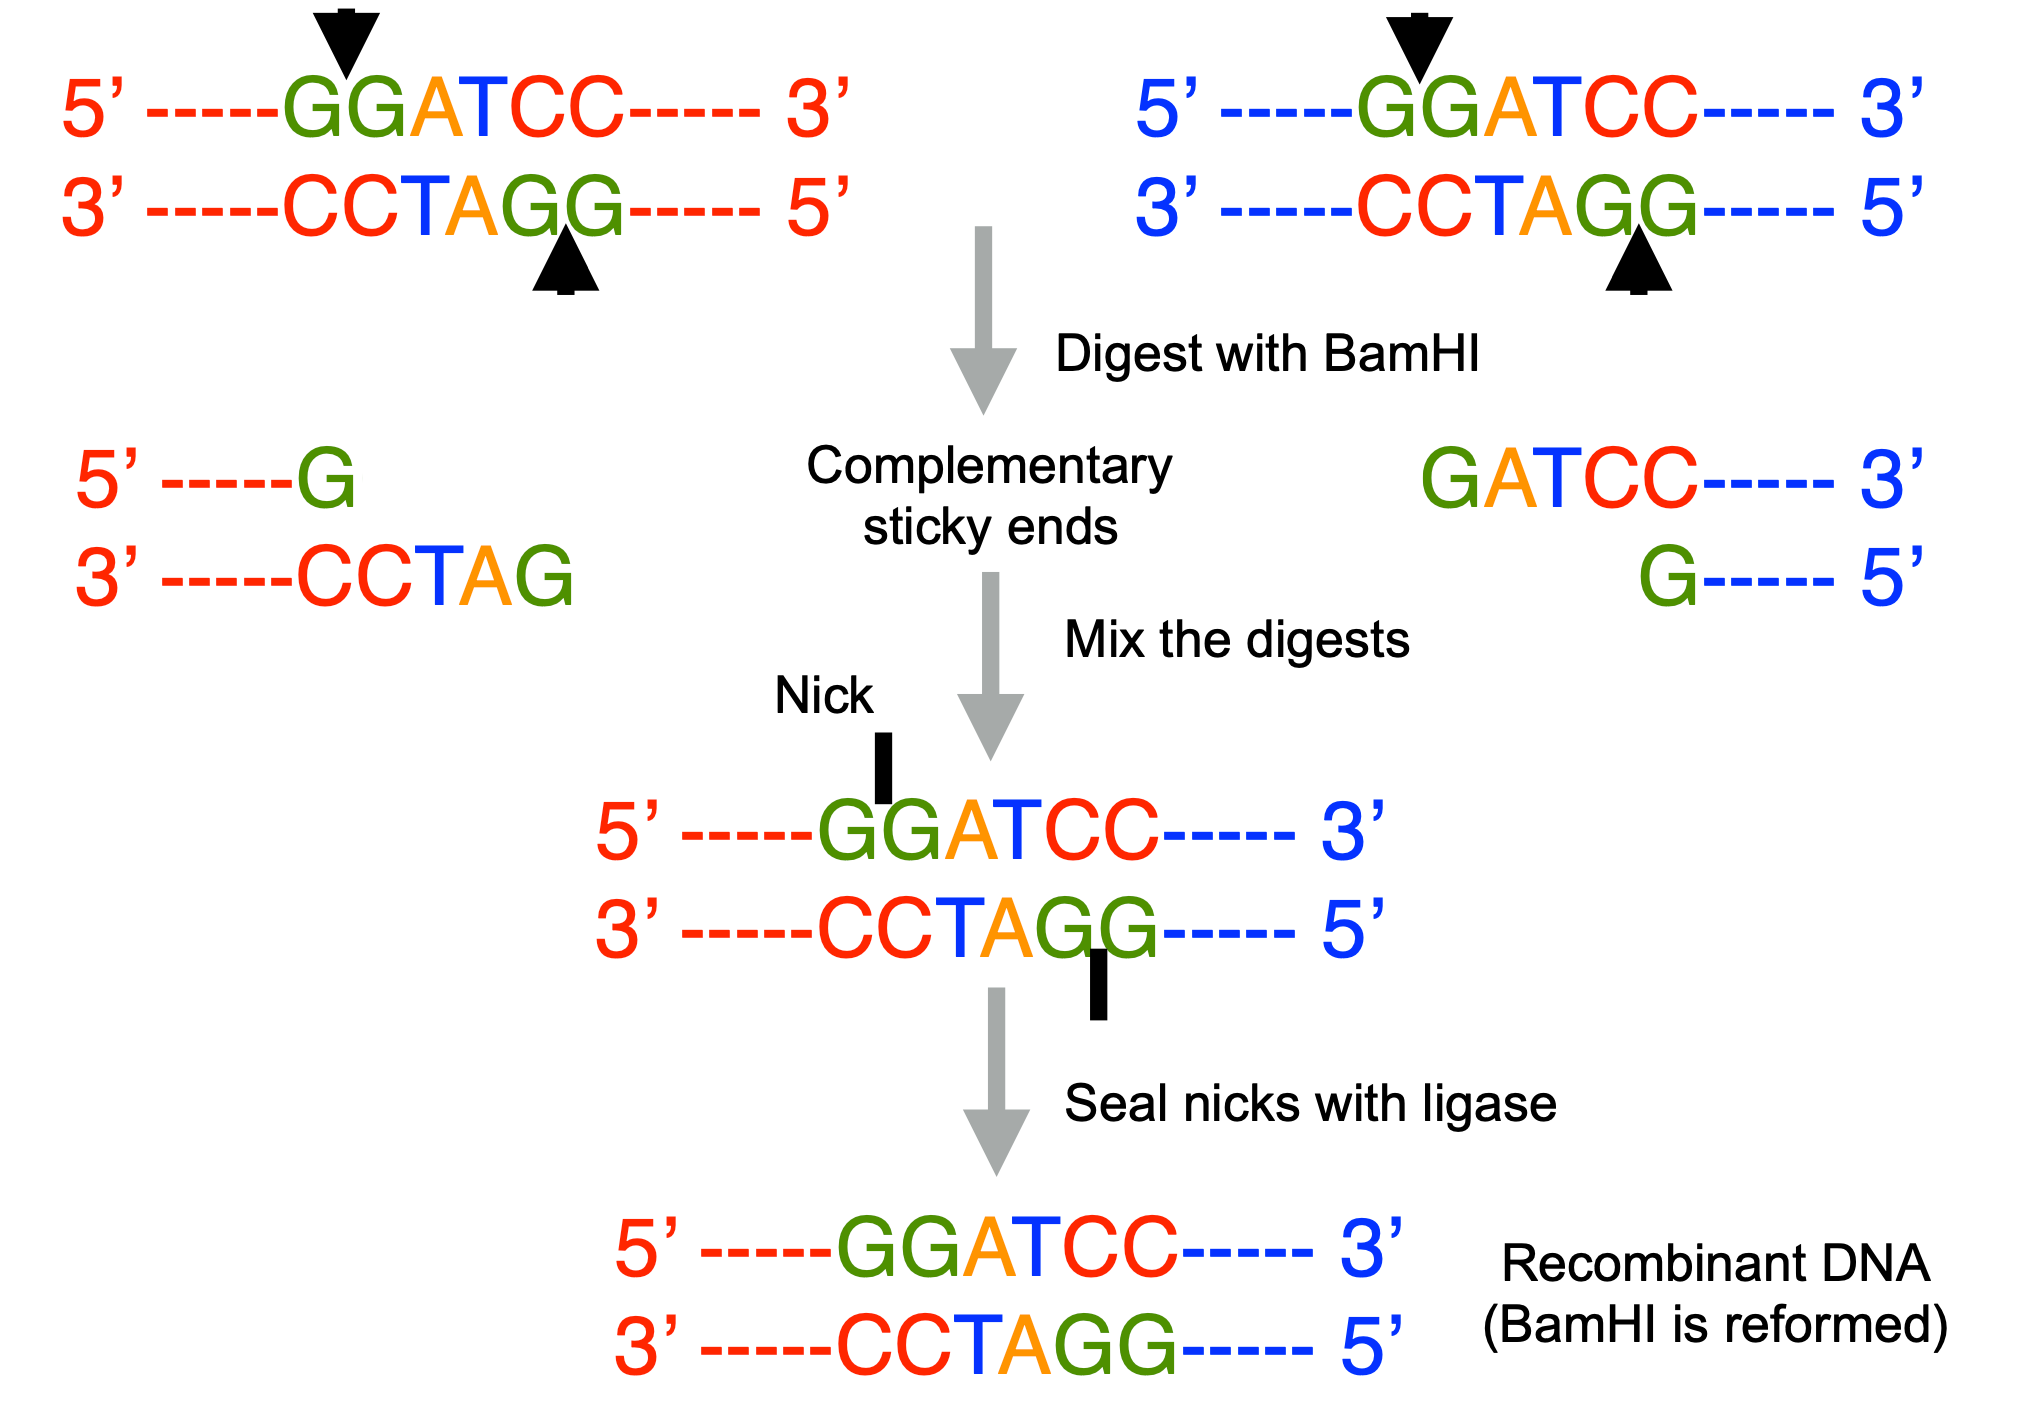
\includegraphics[width=0.8\textwidth]{images/lecture4-2.png}\\[.2in]
\caption{Sequence dependent cleavage and assembly of DNA} 
\label{Fig4-2}
\end{figure}
\subsection{Purifying DNA: Gel elecytophoresis}
\begin{itemize}
    \item DNA is negatively charged in solution at pH=7 to 8.
    \item DNA will \udl{migrate in an electric field}.
    \item Smaller molecules migrate more rapidly in agarose or polyacrylamide gels.
    \item DNA can be visualised in UV light by staining with dyes like \udl{ethidium bromide}.
    \item Can cut out bands from gel in order to purify DNA fragments.
\end{itemize}
\subsection{Inserting DNA into cells: bacterial transformation}
There are two ways to insert DNA liagtion mixture into cells:
\begin{enumerate} 
    \item Chemical transformation:
    \begin{itemize}
        \item wash cells in chilled CaCl\textsubscript{2} to permeabilise the membrane
        \item $ 42\degree$C heat shock to promote DNA uptake
    \end{itemize}
    \item Transformation by electroporation
    \begin{itemize}
        \item wash calls in water (to remove ions)
        \item 5-20kV/cm shock promotes DNA uptake
    \end{itemize}
\end{enumerate}
Both methods are followed by a \udl{recovery period} in rich medium to allow time for \udl{expression of the antibiotic resistance gene}. The cells are plated on \udl{agar plates} containing \udl{nutrients} plus \udl{antibiotics}.
\subsection{Bacterial Cell Culture}
Growth on nutrient agar plates allows \udl{isolation of \textit{colonies}}: a colony is a clone of cells that has grown from one cell.\\[.1in]
Individual colonies are picked into \udl{liquid medium} for growth before preparing DNA. Large scale cultures (thousands to millions of litres) are used for industrial production. Good sterile technique is required.

\subsection{Summary: cloning steps}
Cloning vecors allow foreign DNA to be cloned/amplifies
\begin{enumerate}[itemsep=0mm]
    \item \bd{cut} vector, foreign DNA with compatible restriction enzymes
    \item \bd{isolate} fragments of interest via gel electriphoresis
    \item \bd{ligate} foreign DNA into vector
    \item \bd{transform} recombinant DNA into host (typically \textit{E. coli})
    \item \bd{select} for growth of transformed bacteria
    \item \bd{screen} colonies for correct DNA arrangement
\end{enumerate}
Limitations are
\begin{enumerate} [itemsep=0mm]
    \item Expensive: it requires very highly purifies enzymes.
    \item Chance/Need more control: it requires restriction sites in the right place.
\end{enumerate}

\section{CRISPR/cas9}
\subsection{CRISPR/cas9: programmable recognition}
The gRNA specificity is 20 bases, which ensures the accuracy of editing. Target must be followed by
protospacer adjacent motif (PAM) = NGG for S. pyogenes Cas9.\\[.2in]
\begin{figure}[h]
\centering
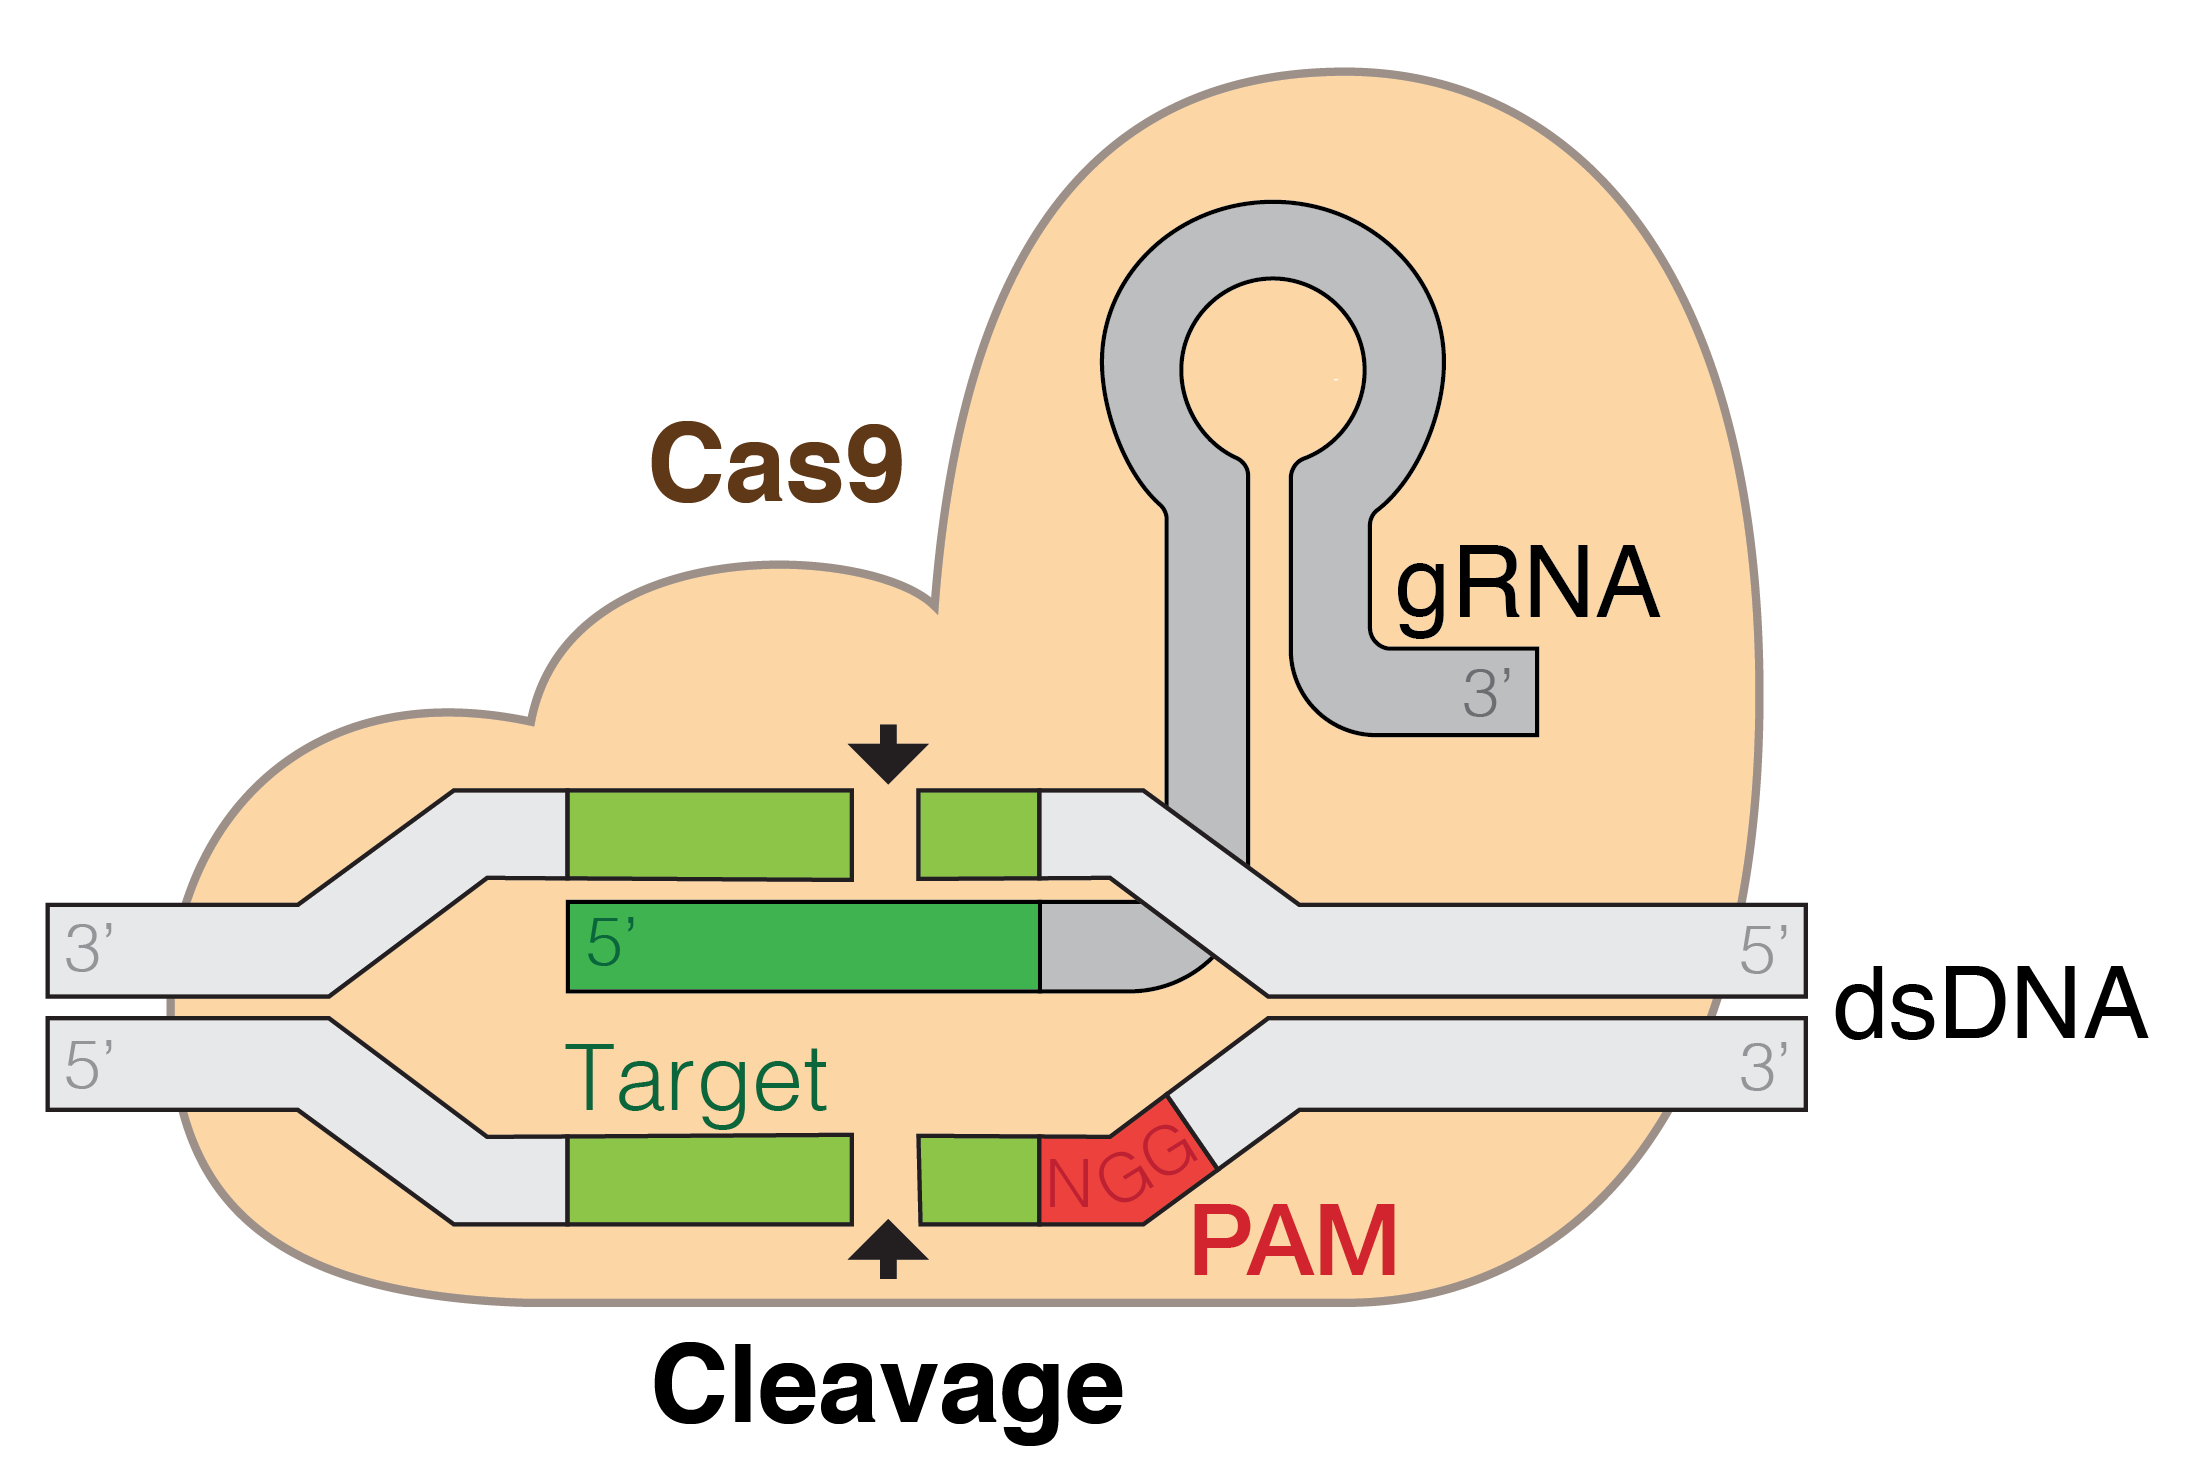
\includegraphics[width=0.6\textwidth]{images/GRNA-Cas9.png}\\[.2in]
\caption{CRISPR/cas9}
\end{figure}
In the Non-Homologous End Joining (NHEJ) (figure \ref{repair}), one can knock out the gene by making a cut at the specific location and causes deletion and insertions which disable the gene.\\[.2in]
Even more powerfully, by transforming a piece of \udl{linear DNA} containing the desired changes. If the linear DNA has sequence similarities on either side of the cut side, the repair machinery will do the Homology Directed Repair (HDR) by reference with the linear DNA inserted. This is why it is very efficient in editing the genes.
\begin{figure}[h]
\centering
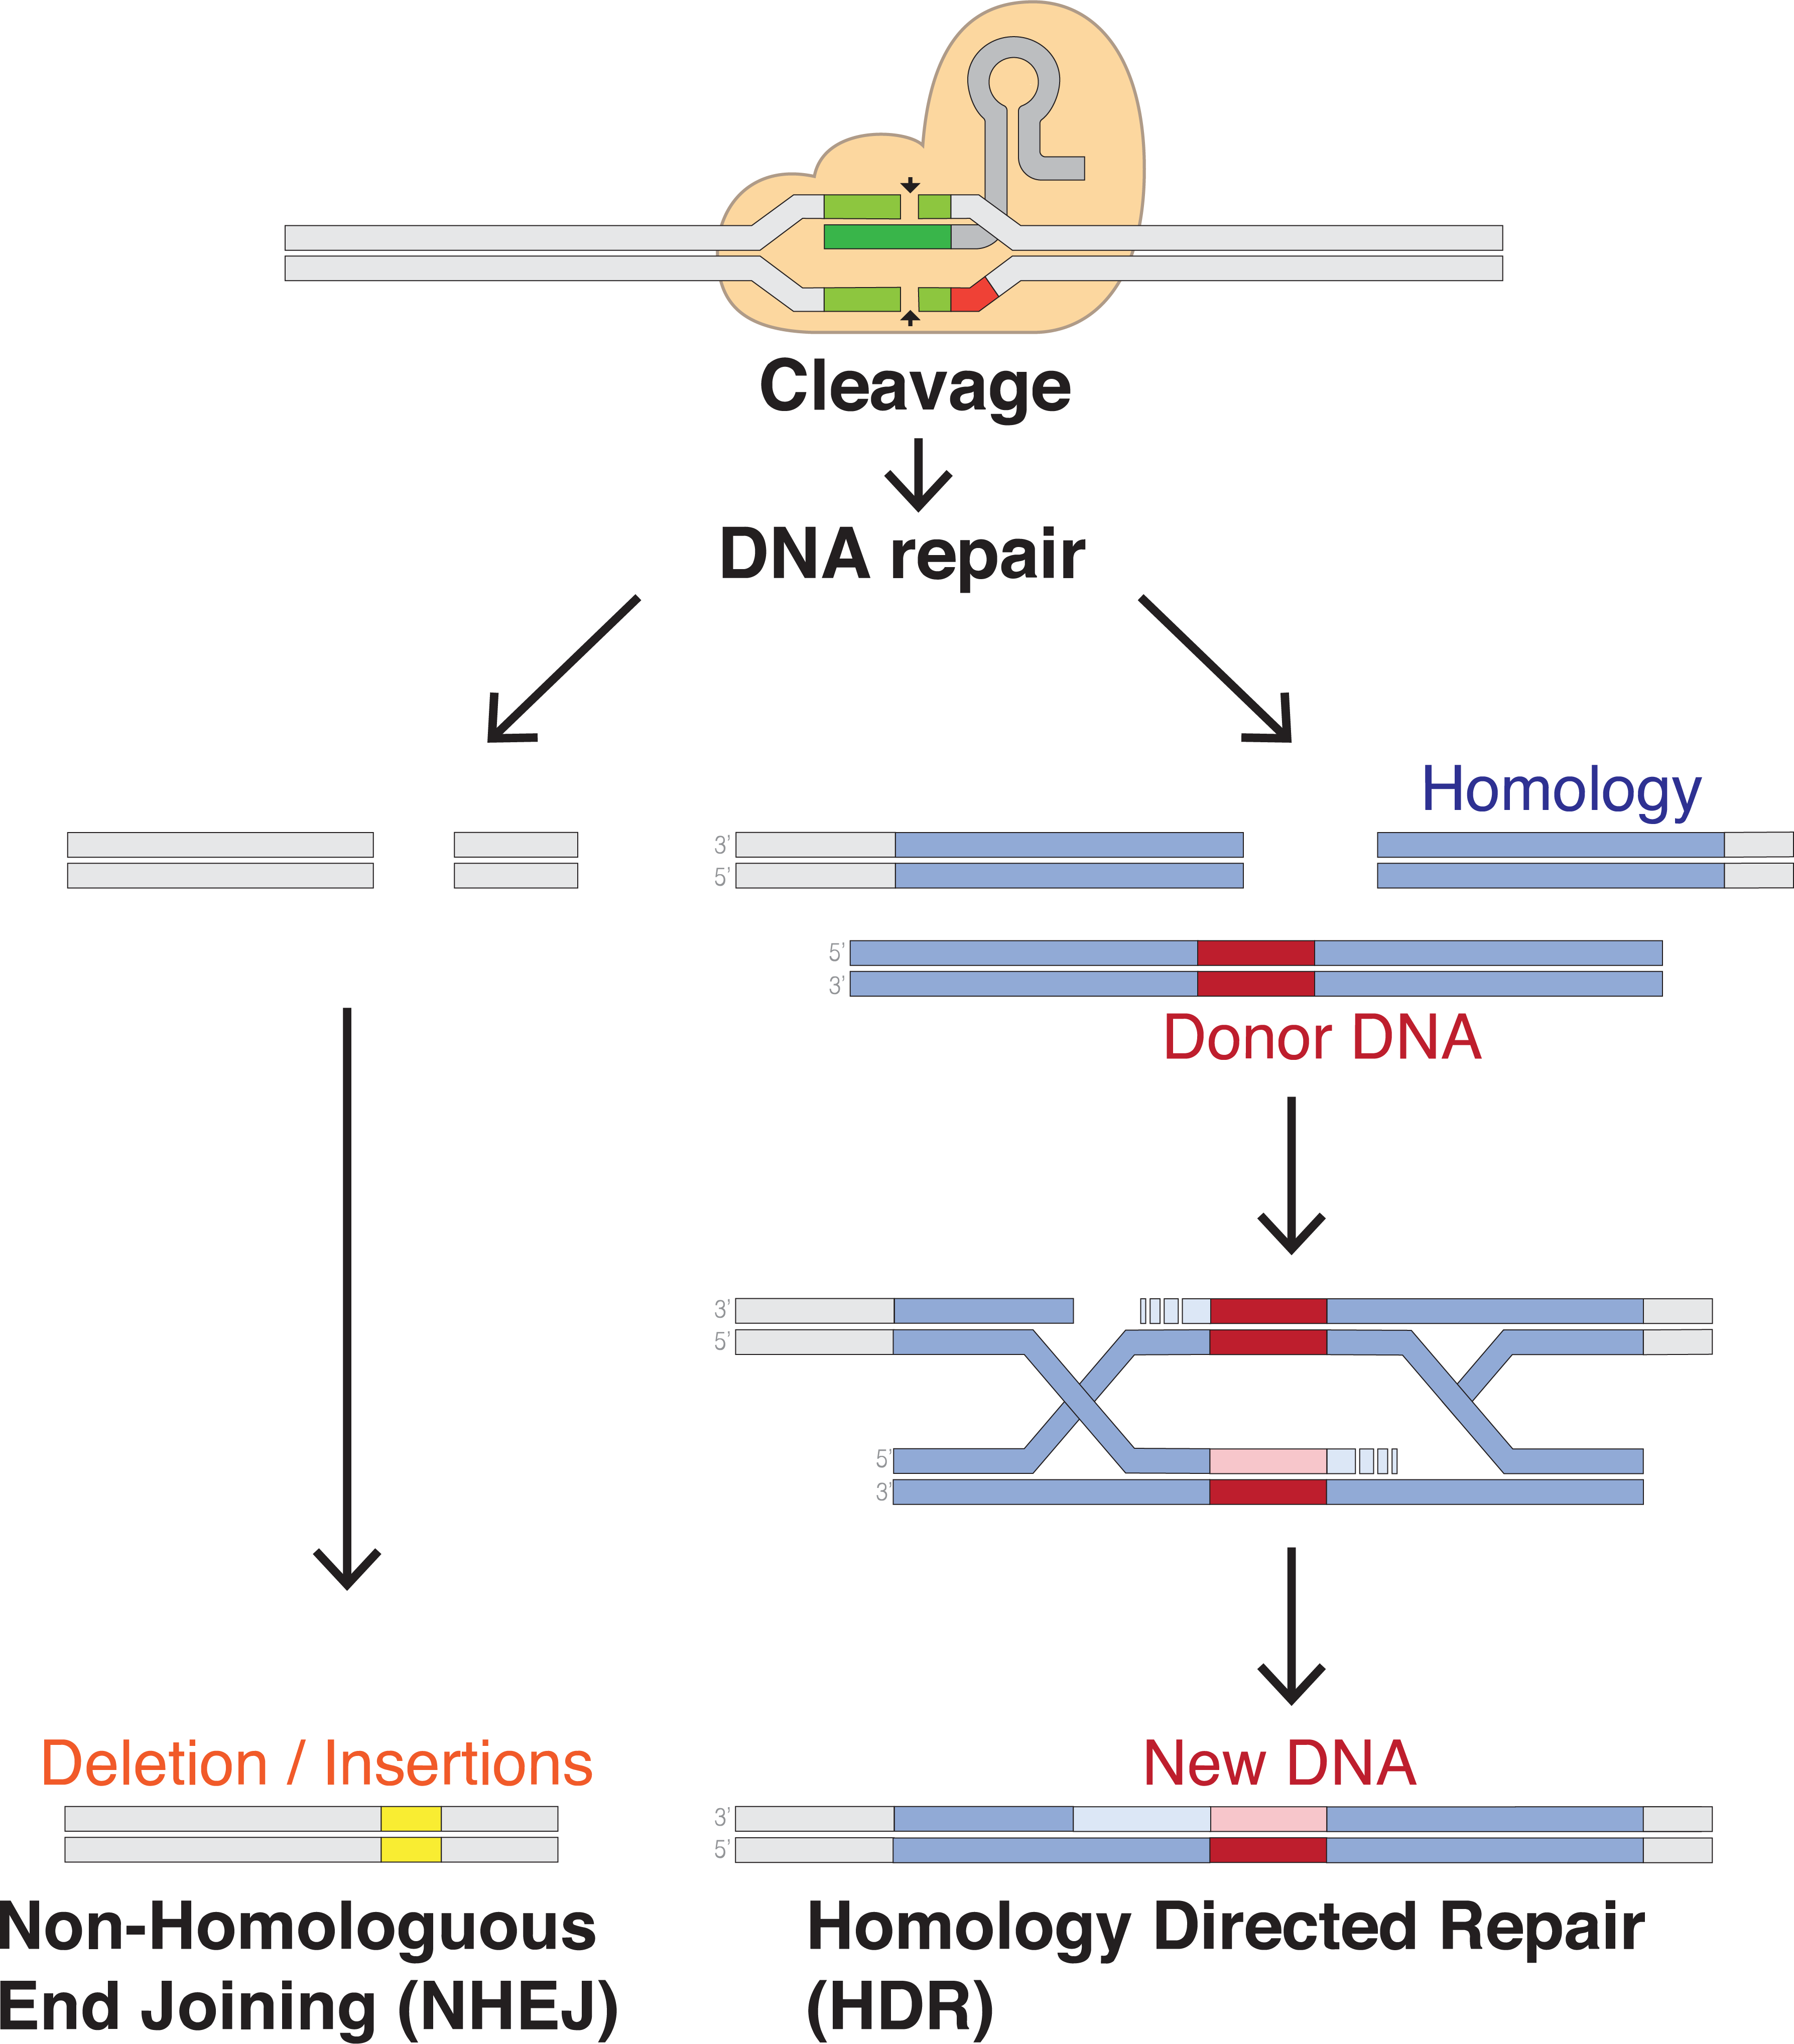
\includegraphics[width=0.4\textwidth]{images/DNA_Repair.png}\\[.2in]
\caption{DNA repair with CRISPR/cas9}
\label{repair}\\[.2in]
\end{figure}
\subsection{Application areas}
\begin{itemize}
    \item programmable sequence-specific nucleases
    \item simpler genome editing: potential to reverse genetic diseases
    \item programmable transcription regulators
    \item systematic whole-genome mutagensis (allows functional screens)
    \item transgenic mice much more quickly
    \item dCas9 mutant does not cut (figure \ref{dCas9})
\end{itemize}
\begin{figure}[h]
\centering
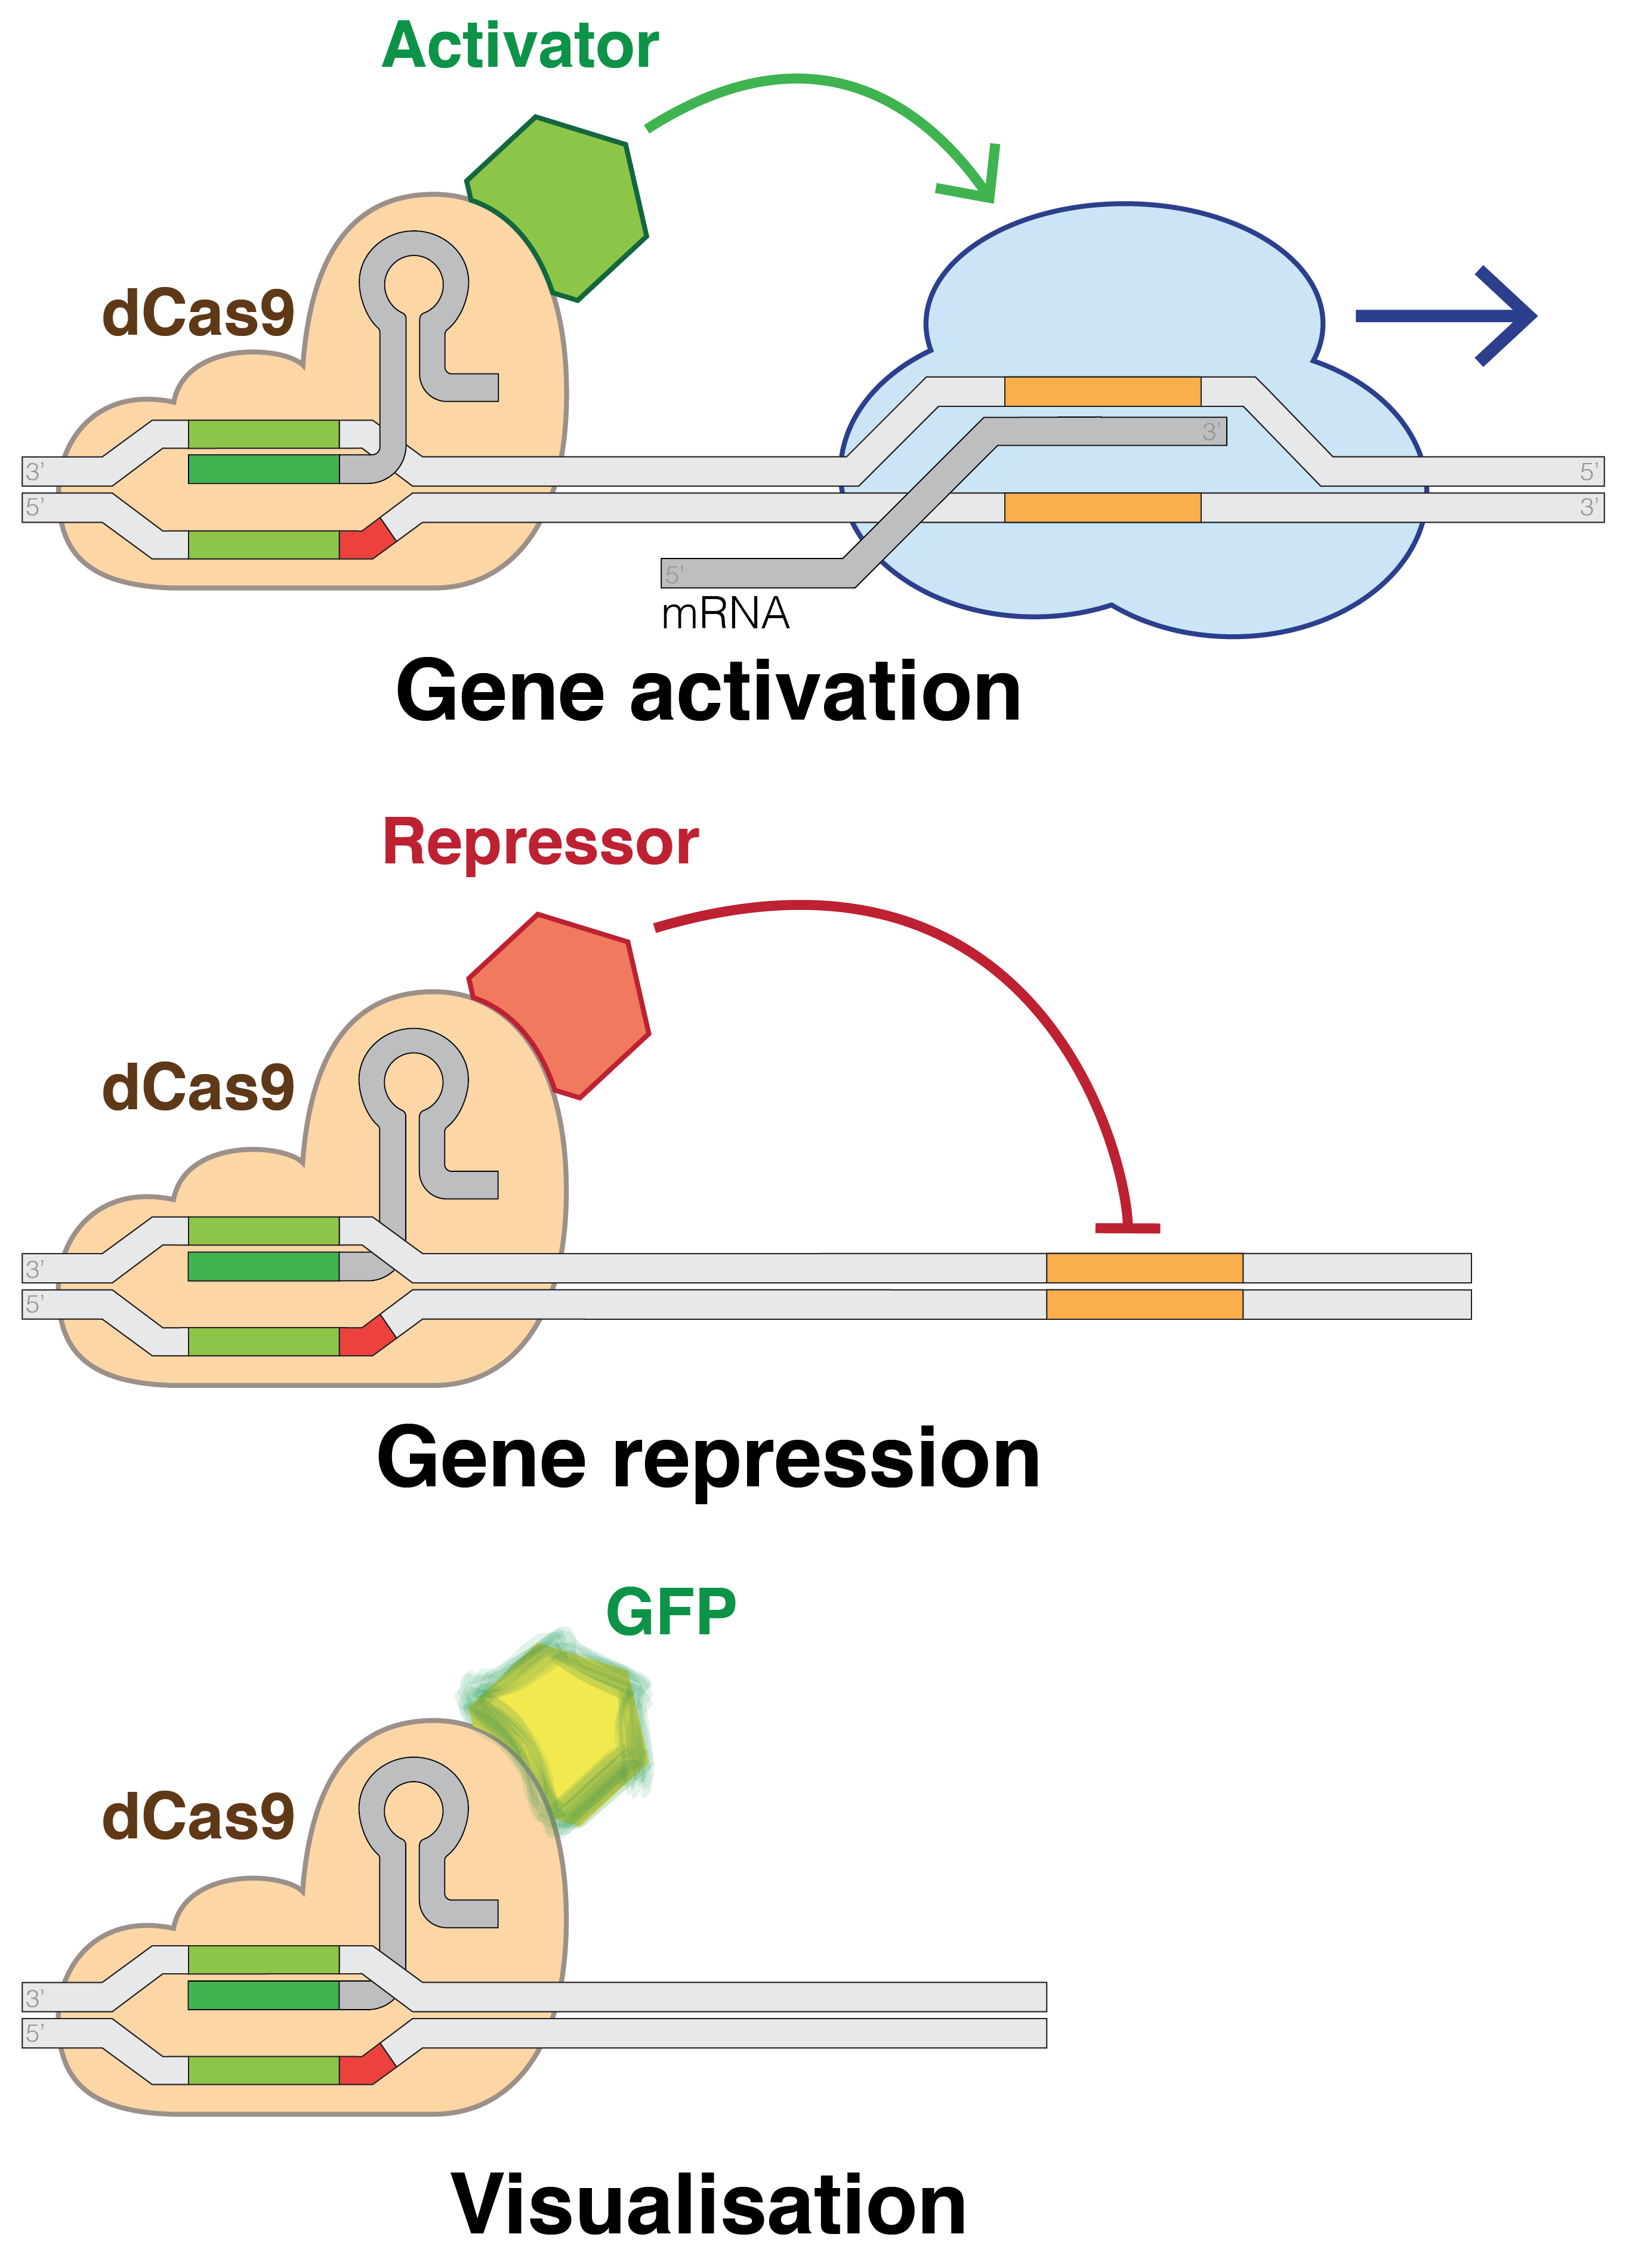
\includegraphics[width=0.4\textwidth]{images/Dead-Cas9_potential_applications.png}\\[.2in]
\caption{dCas9 Potential Application}
\label{dCas9}
\end{figure}
\section{Polymerase Chain Reaction (PCR)}
PCR can \udl{amplify} a single DNA template molecule into $10^9$ copies in a few hours (30 doublings).\\[.2in]
Recall that DNA polymerases extend a 3'-OH in the 5' to 3' direction. The 3'-OH can be on a synthetic DNA primer. DNA base pairing and thus primer annealing is \udl{temperature dependent}.\\[.2in]
PCR creates billions of copies of a region of interest. The region of interest is \udl{defined by synthetic DNA primers}.
\subsection{Reaction Mix and Reaction}
\bd{Reaction mix}
\begin{itemize}
    \item DNA template
    \item Primers complementary to the ends of the target region
    \item dNTPs (i.e. dATP, dCTP, dGTP, dTTP)
    \item Buffer, salts to keep the polymerase happy
    \item Thermotolerant DNA polymerase (e.g. Taq, phusion etc)
\end{itemize}
\bd{Reaction}\\[.1in]
\udl{Thermocycler} is programmed to cycle the temperature
\subsection{Engineering with PCR}
Engineering with restriction enzymes can be hard, where PCR can make things easier.\\[.2in]
Advantages:
\begin{itemize}
    \item Can isolate fragments independently of restriction sites
    \item Can fuse fragments independently of restriction sites
\end{itemize}
Limitations:
\begin{itemize}
    \item length of target region
    \item error rate of DNA polymerase
    \item high \%GC regions
\end{itemize}
\subsection{Seamless joining of DNA fragments with PCR}
\begin{enumerate}
    \item PCR - amplifying left fragment
    \begin{figure}[h]
    \centering
    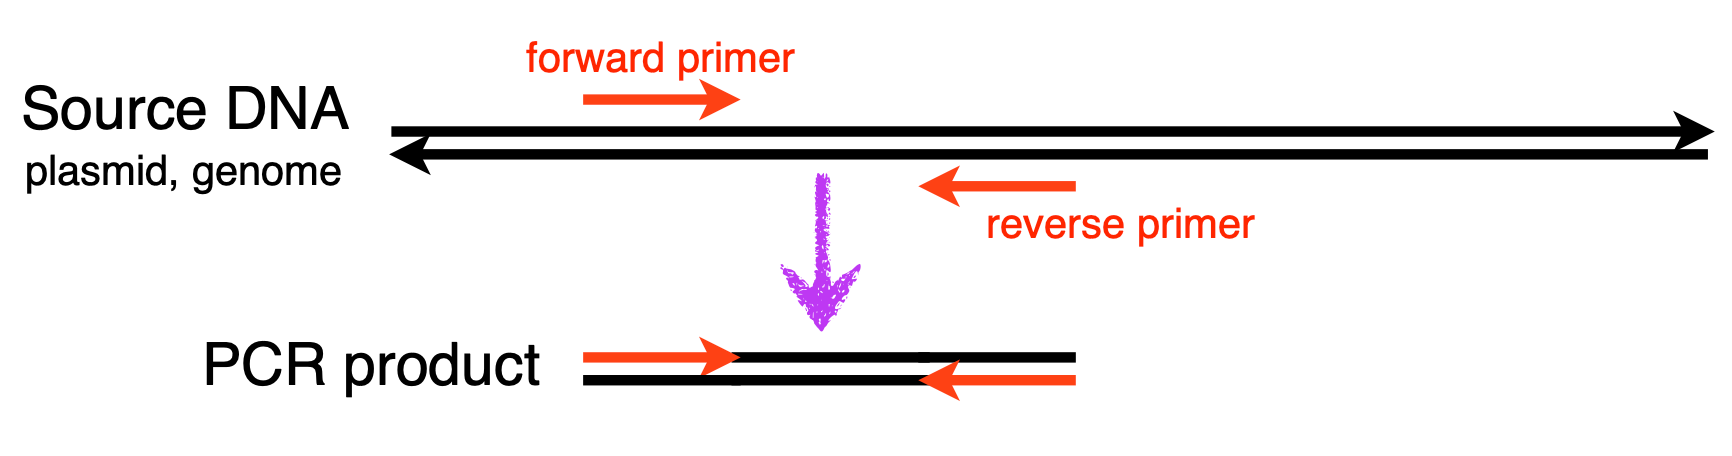
\includegraphics[width=0.6\textwidth]{images/4-3-1.png}\\[.2in]
    \caption{Step 1 - PCR amplifying left fragment}
    \end{figure}
    \item PCR - amplifying right fragment: N.B. \udl{forward primer} contains \udl{same sequence} as end of Step 1 PCR product.
    \begin{figure}[h]
    \centering
    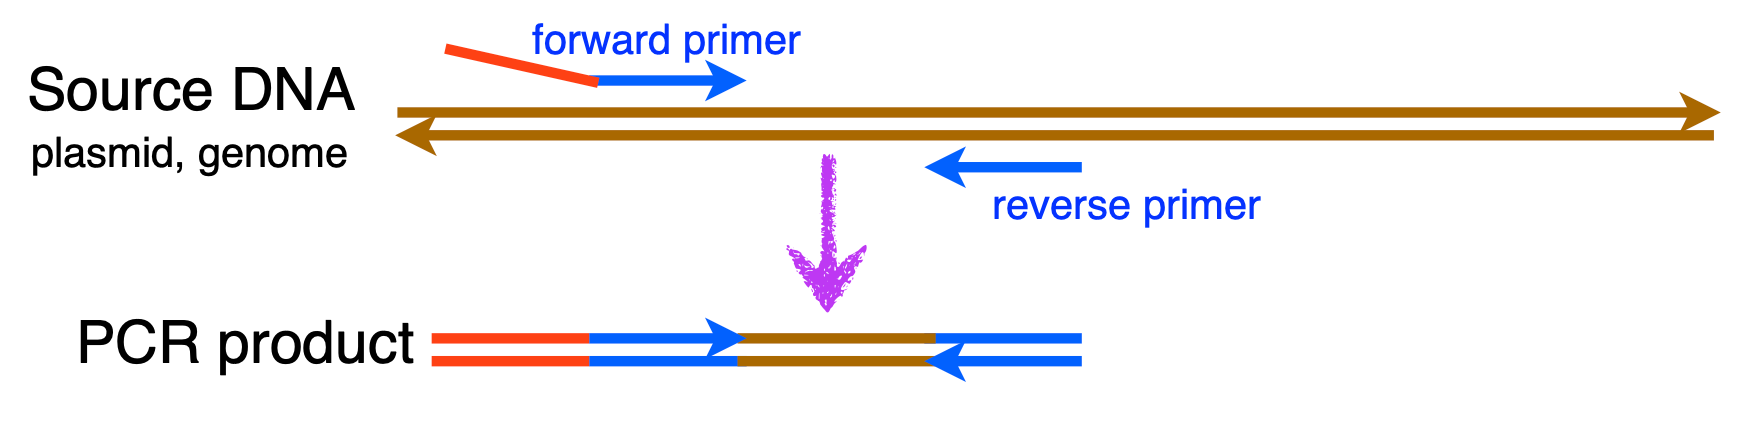
\includegraphics[width=0.6\textwidth]{images/4-3-2.png}\\[.2in]
    \caption{Step 2 - PCR simplifying right fragment}
    \end{figure}
    \item PCR reaction using products from steps 1 + 2 mixed together
    \begin{figure}[h]
    \centering
    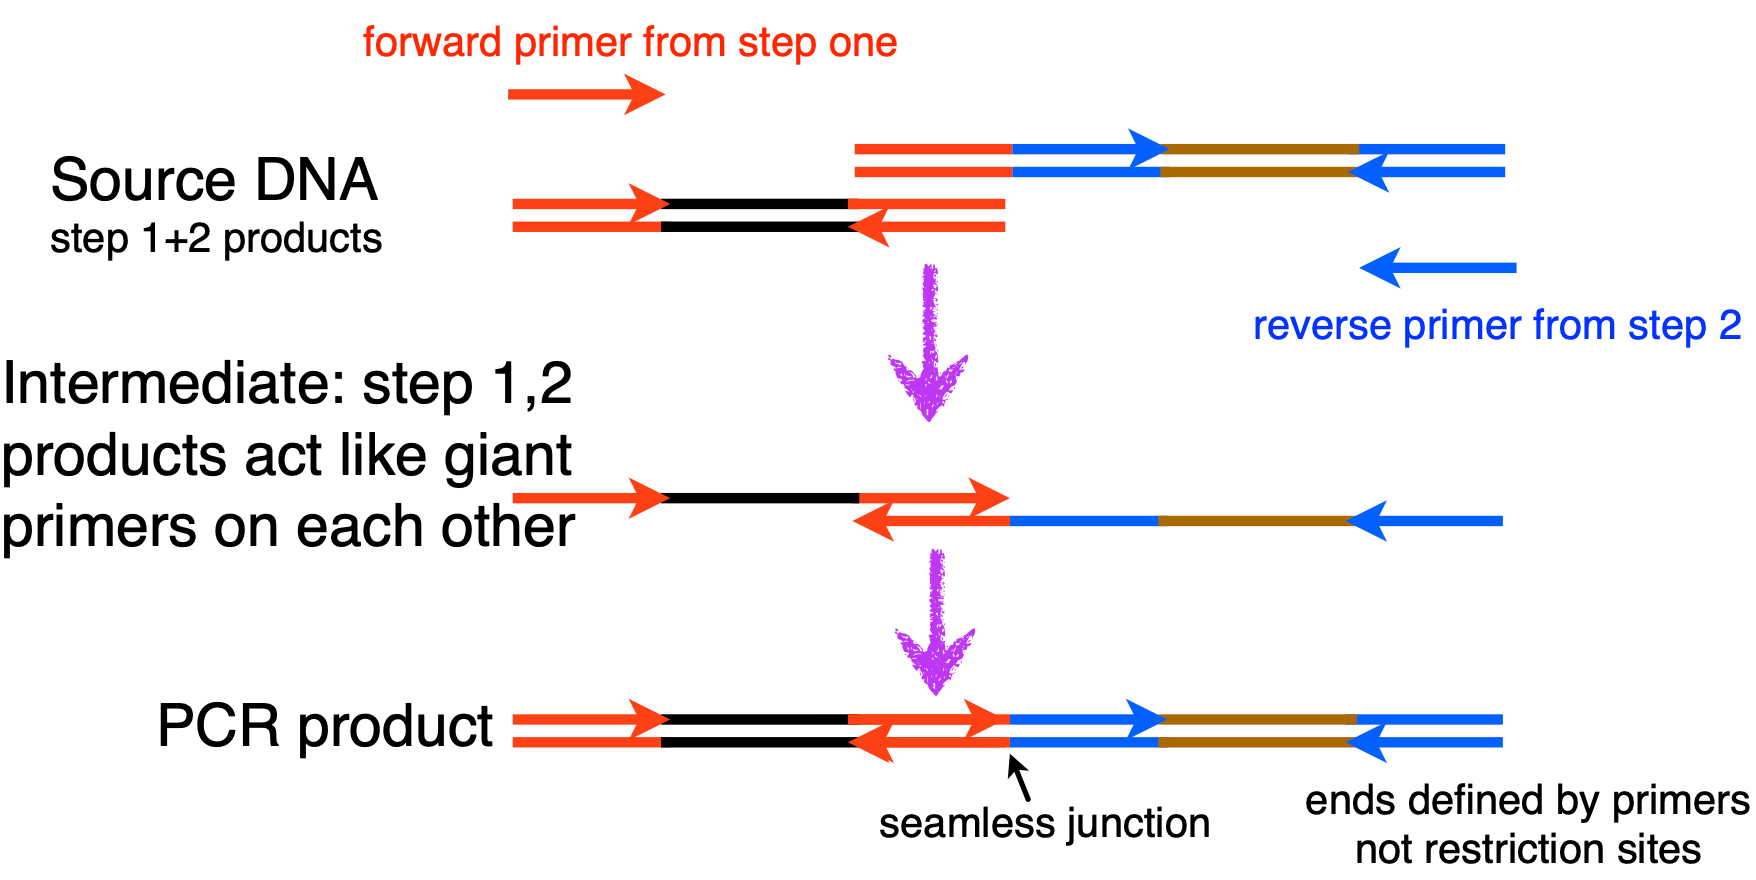
\includegraphics[width=0.6\textwidth]{images/4-3-3.png}\\[.2in]
    \caption{Step 3 - PCR reaction using products from step 1 and 2}
    \end{figure}
\end{enumerate}
\subsection{Things that can go wrong with PCR}
Assume fresh and correct buffers and enzymes and that thermocycler is programmed correctly.
\begin{itemize}
    \item No product: check primer design, decrease annealing temperature, vary MgCl\textsubscript{2} levels.
    \item Multiple products: check primer design, use hot start enzyme, increase annealing temperature, vary MgCl\textsubscript{2} levels.
    \item Product in negative control: contamination (use laminar air flow hood, filter tips).
    \item Primer dimers\footnote{primers self-prime or prime on each other}: redesign primers.
\end{itemize}

\section{Gibson Assembly}
Limitations:
\begin{itemize}
    \item Few. Cost for 100,0000 base scale synthesis
    \item T5 exonuclease will destroy small fragments
\end{itemize}
Advantage:
\begin{itemize}
    \item seamless joining of arbitrary DNA fragments
    \item multiple fragments can be joined in one step
    \item currently cheaper than de novo synthesis
\end{itemize}

\section{De novo synthesis}
Advantage:
\begin{itemize}
    \item independent of restriction enzymes
    \item independent of ability to PCR fragment of interest
    \item allows complete resign of DNA sequence
\end{itemize}
Limitations:
\begin{itemize}
    \item cost (but dropping rapidly)
    \item Scale: ~1kb fragments are ordered by many labs
\end{itemize}
N.B. Small scale sythesis of ~20-50nt DNA oligonucleotides\footnote{a polynucleotide whose molecules contain a relatively small number of nucleotides.} underpins PCR (the primers), DNA sequencing (the primer).